\section{RA5}
\subsection*{Resultados de aprendizaje}
Identificar los conceptos básicos de análisis de algoritmos para examinar un conjunto básico de ellos considerando el tiempo de ejecución.

\subsection*{Contenido según programa}
Unidad 4: Introducción a la programación estructurada.  Interpretación de enunciados. Ideas sobre programas y datos.  Algoritmos. Estructuras básicas de programación.  Secuencia. Selección.  Iteración. Salto incondicional. Eliminación del salto incondicional.  Primer paradigma de programación; programación estructurada.  Diagramas de flujo del programa: símbolos de operación, comentarios, decisión, líneas de flujo, conexión. Pseudocódigo.  Implementación de algoritmos sencillos.

Unidad 5. Control de flujo en lenguaje C.  Implementación de la Estructura de Selección: Simple (if). Doble (if-else).  Múltiple (switch-case).  Estructura de Repetición: Ciclos while, do-while, y for.  Sentencias break y continue. Bucles anidados.  Control de flujo con el preprocesador: compilación condicional. Implementación de algoritmos en lenguaje C.

%--------------------------------------------------------------------------------
%--------------------------------------------------------------------------------
\subsection*{Introducción a la programación estructurada.}
\subsection*{Repaso}

\begin{minipage}{0.5\textwidth}
  \textbf{si} \it{condición} \textbf{entonces}\\
  \hspace*{10mm}\it{proceso}\\
  \textbf{fin si}\\
\end{minipage}
\begin{minipage}{0.5\textwidth}
\center
  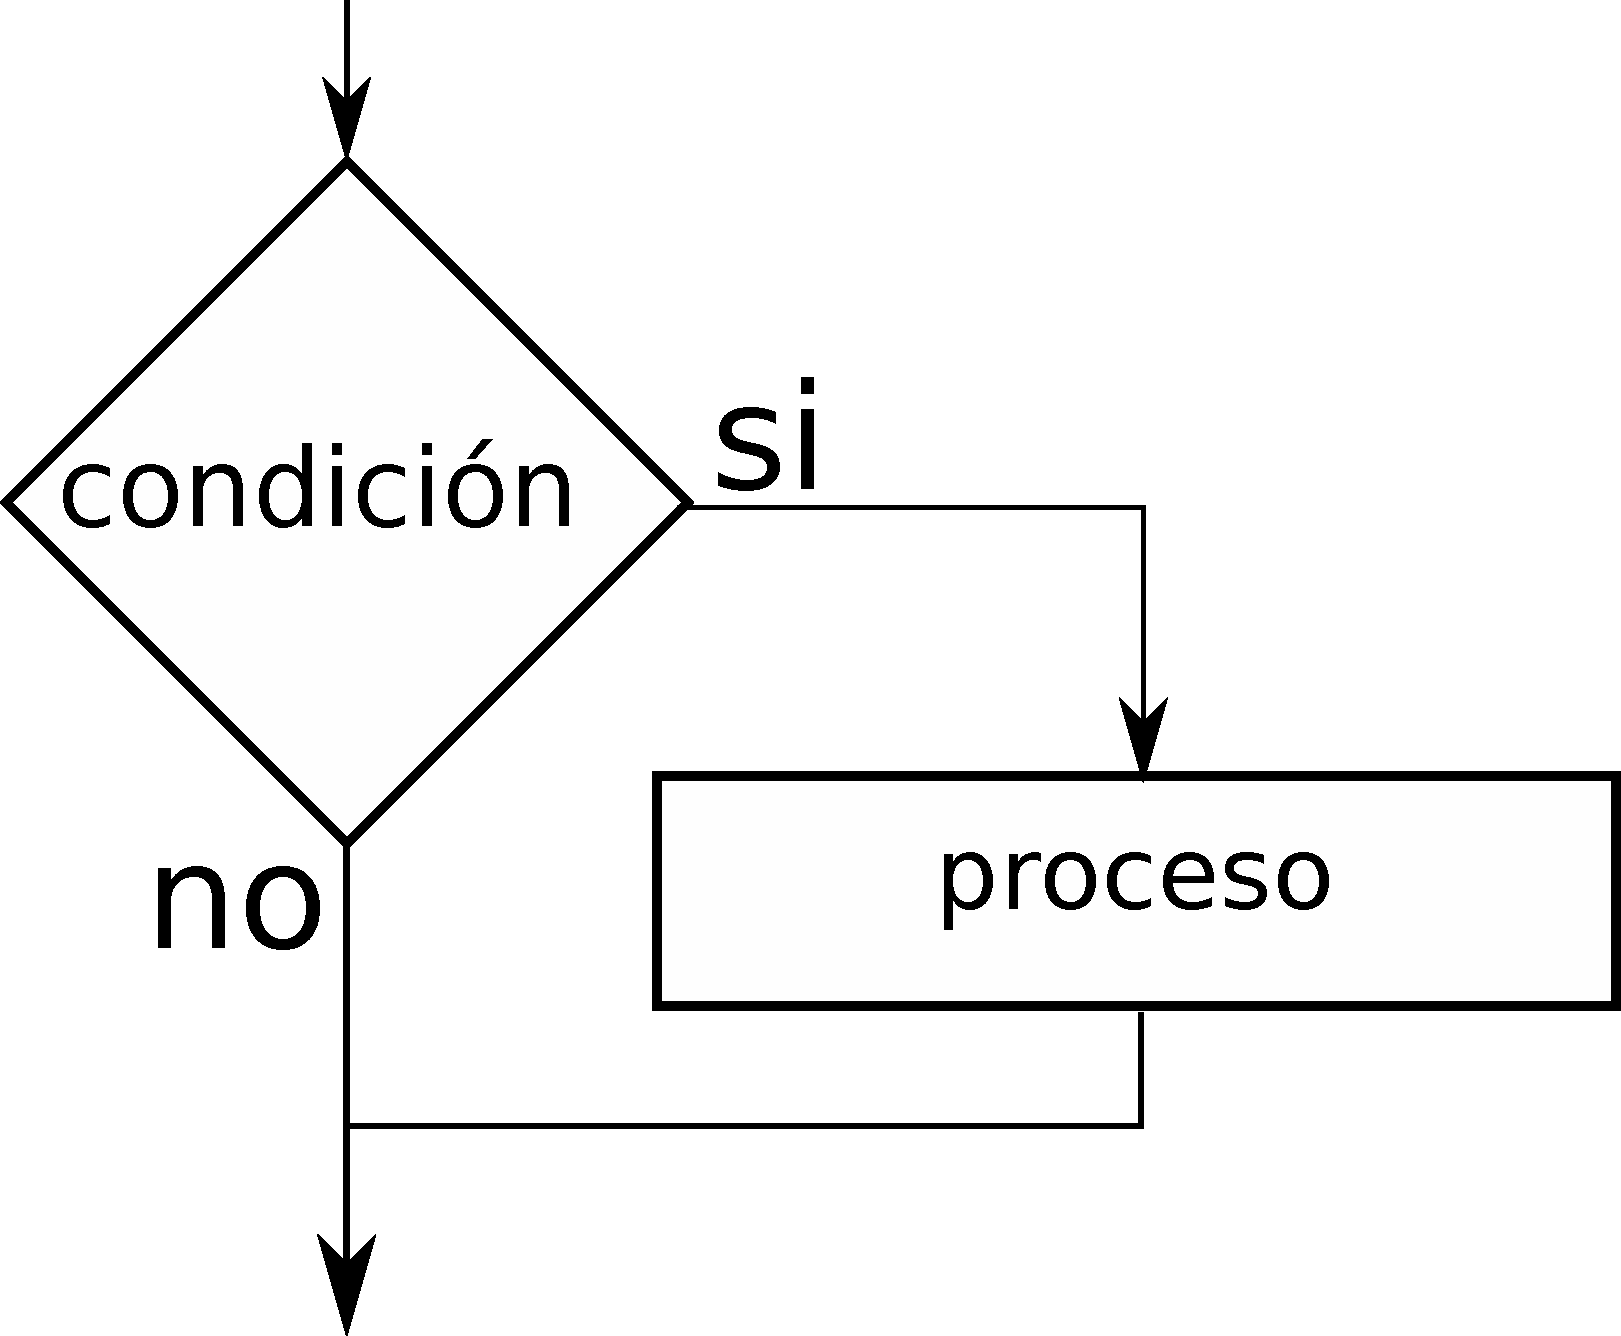
\includegraphics[height=40mm]{img/if.pdf}
\end{minipage}

\vspace{10mm}

\begin{minipage}{0.5\textwidth}
  \textbf{si} \it{condición} \textbf{entonces}\\
  \hspace*{10mm}\it{proceso 1}\\
  \textbf{si no}\\
  \hspace*{10mm}\it{proceso 2}\\
  \textbf{fin si}\\
\end{minipage}
\begin{minipage}{0.5\textwidth}
  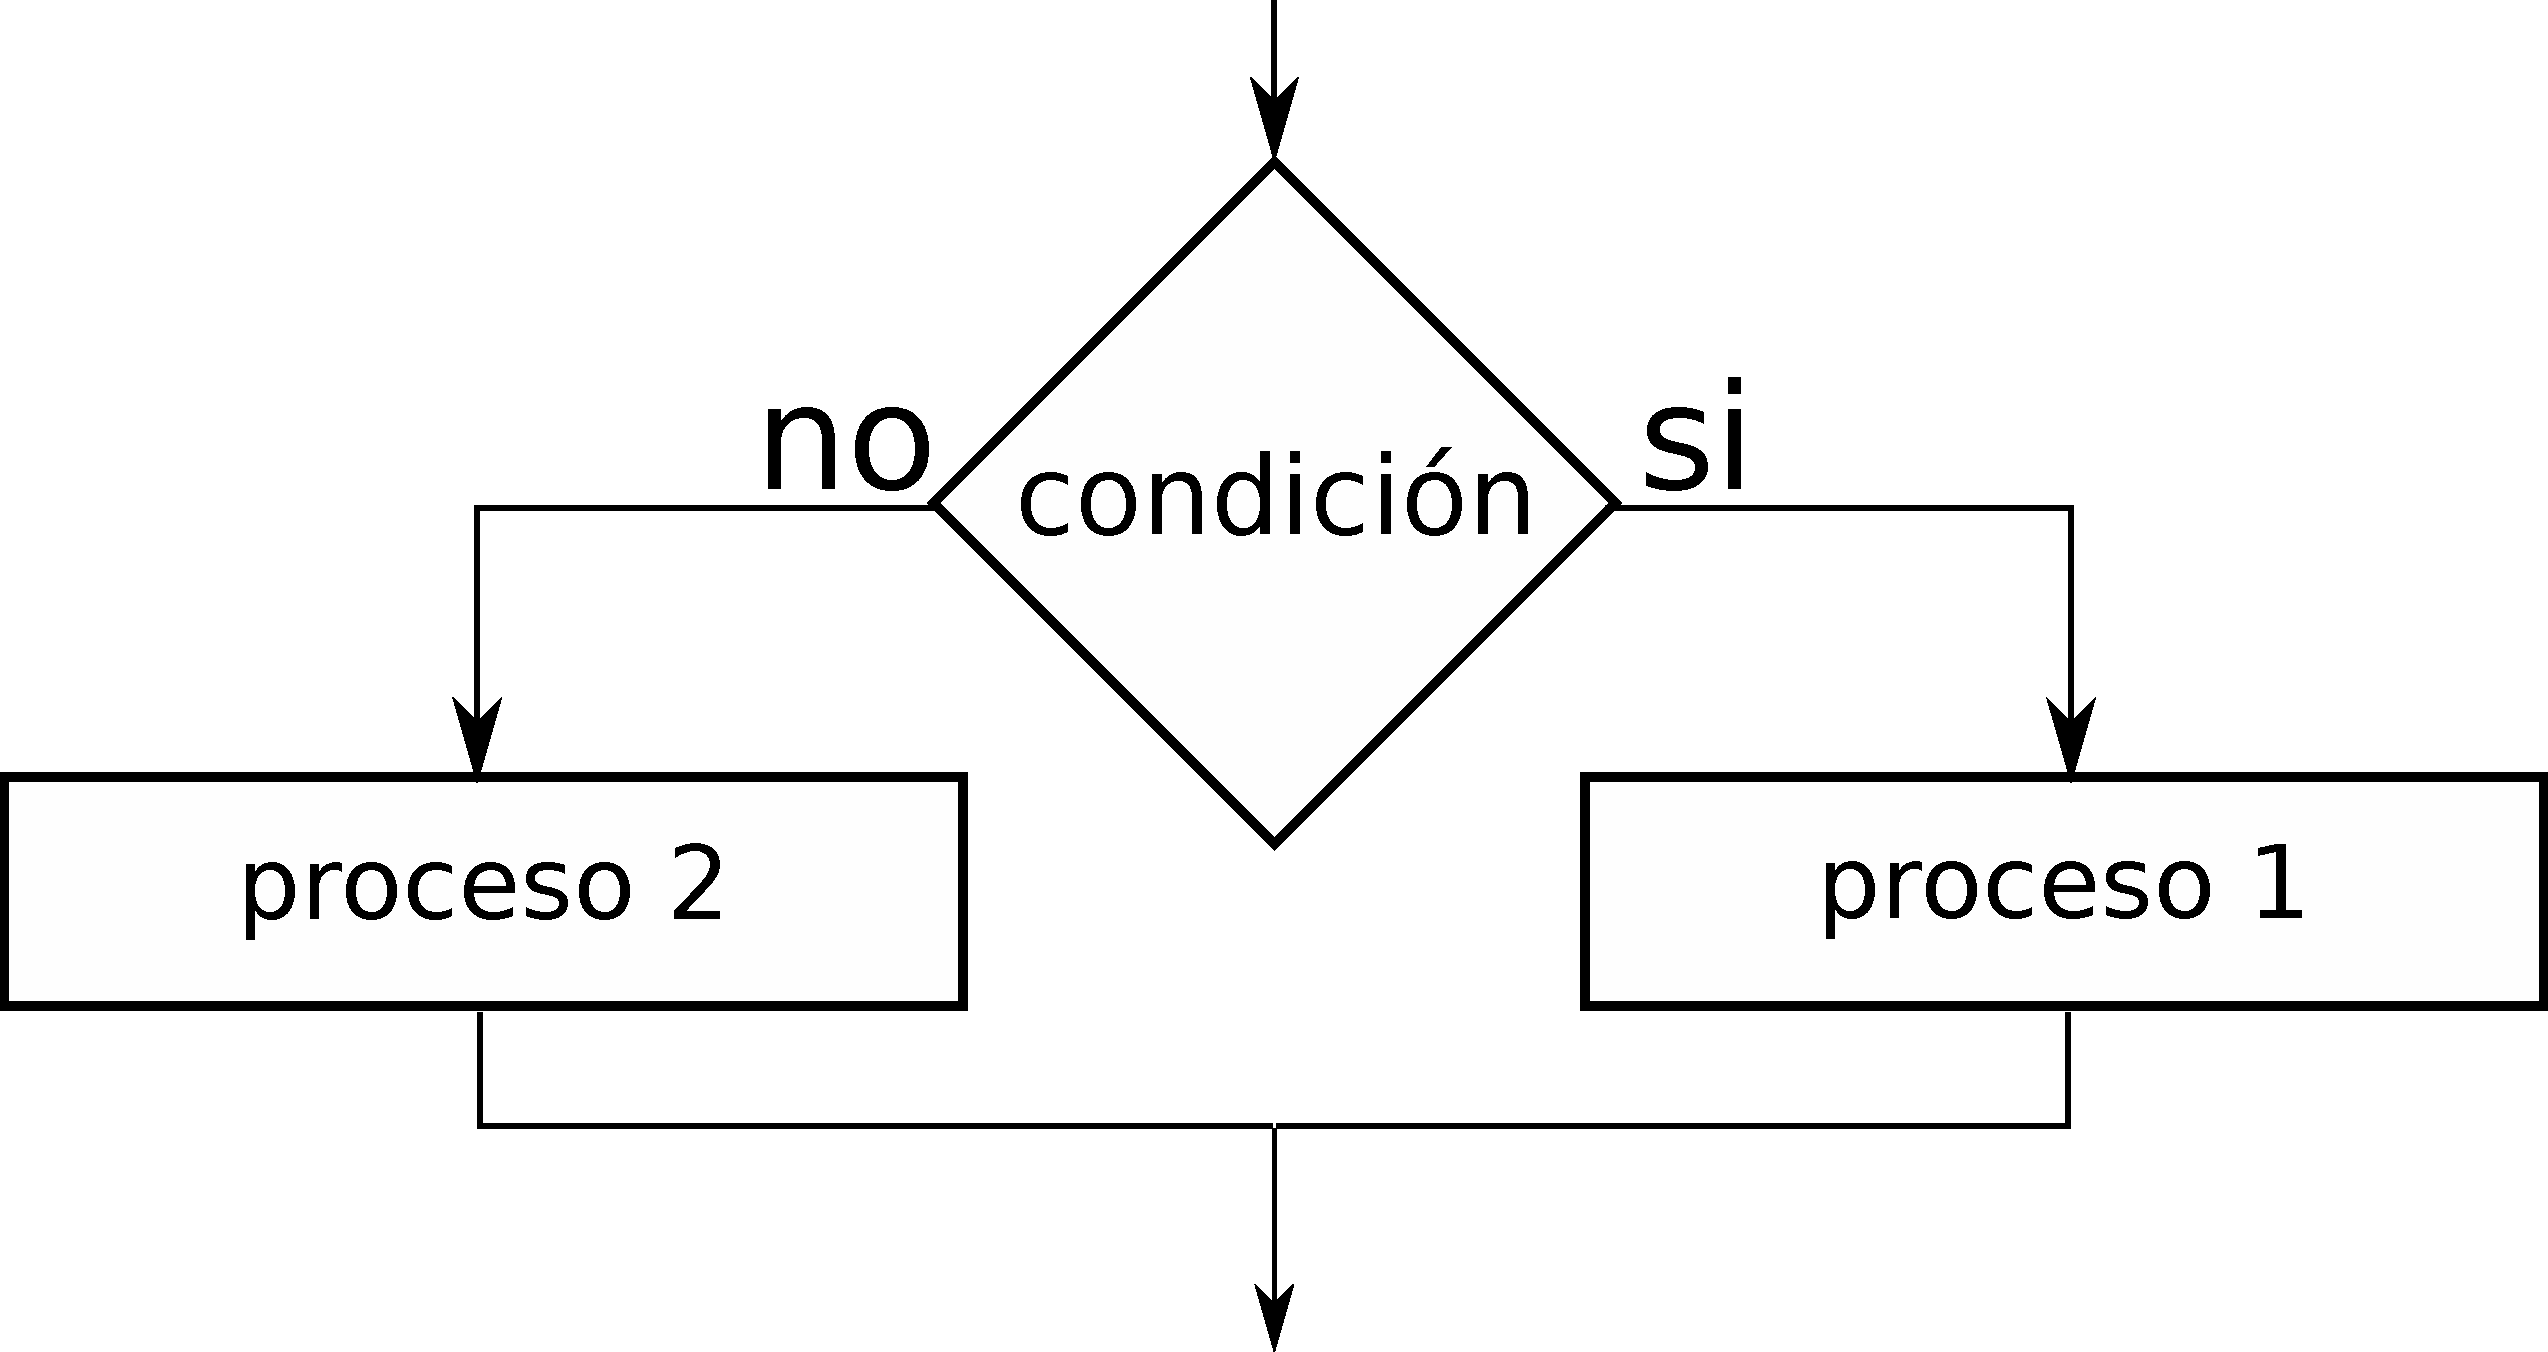
\includegraphics[height=40mm]{img/if_else.pdf}
\end{minipage}

\vspace{10mm}

\begin{minipage}{0.5\textwidth}
  \textbf{mientras} \it{condición} \\
  \hspace*{10mm}\it{proceso}\\
  \textbf{fin mientras}\\
\end{minipage}
\begin{minipage}{0.5\textwidth}
\center
  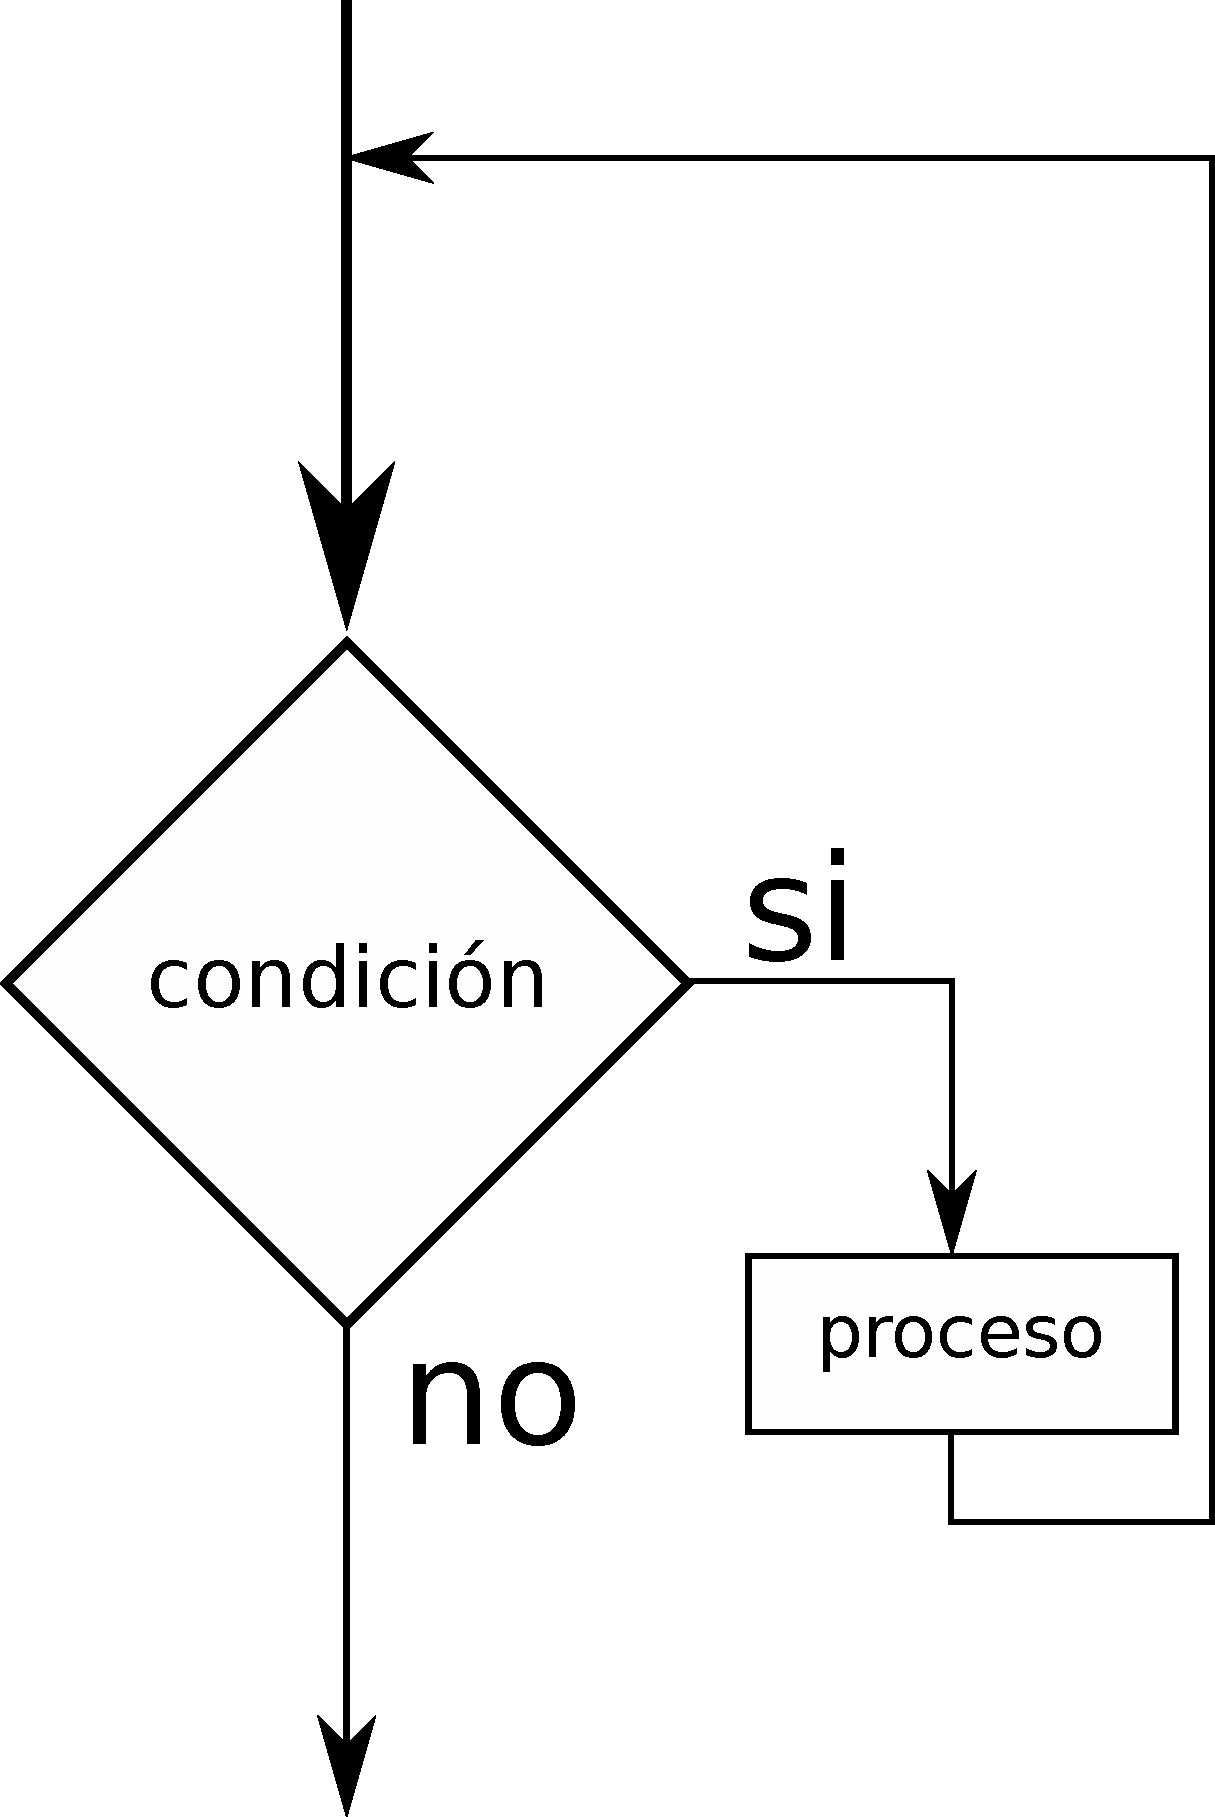
\includegraphics[height=40mm]{img/mientras.pdf}
\end{minipage}

\vspace{10mm}

\begin{minipage}{0.5\textwidth}
  \textbf{hacer} \\
  \hspace*{10mm}\it{proceso}\\
  \textbf{mientras} \it{condición}\\
\end{minipage}
\begin{minipage}{0.5\textwidth}
\center
  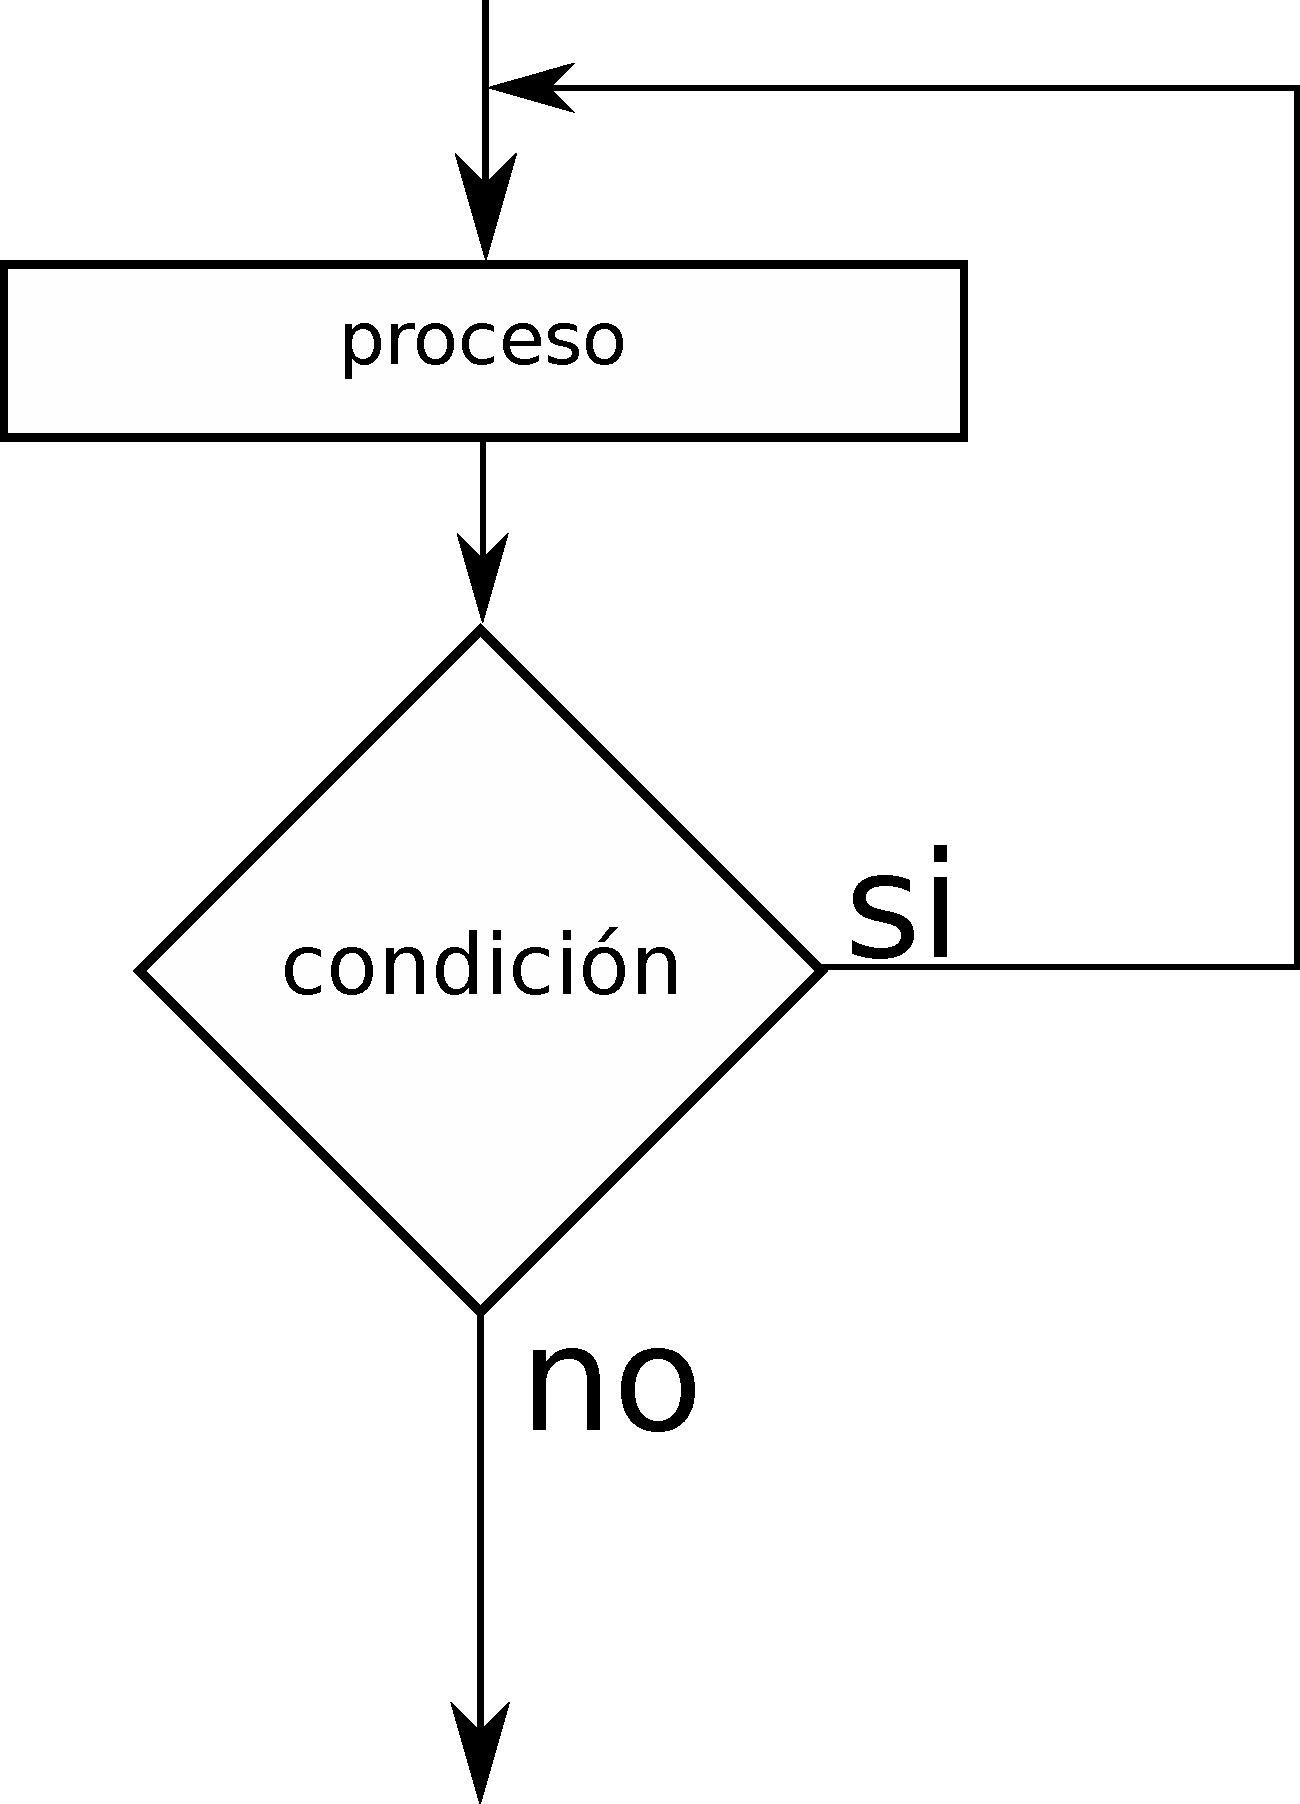
\includegraphics[height=40mm]{img/hacer_mientras.pdf}
\end{minipage}

%--------------------------------------------------------------------------------
%--------------------------------------------------------------------------------
\setcounter{subsection}{4}
\subsection{Ejercicios:}
Realizar un programa que solicite la dimensión en cm de lados de un rectángulo y muestre la superficie del mismo

\subsubsection*{Solución}
\begin{lstlisting}[style=pseudocodigo]
imprimir: Ingrese la longitud del primer lado
leer:lado1
imprimir: Ingrese la longitud del segundo lado
leer: lado2
superficie = lado1 * lado2
imprimir: superficie
\end{lstlisting}

\begin{figure}[h!]
  \centering
  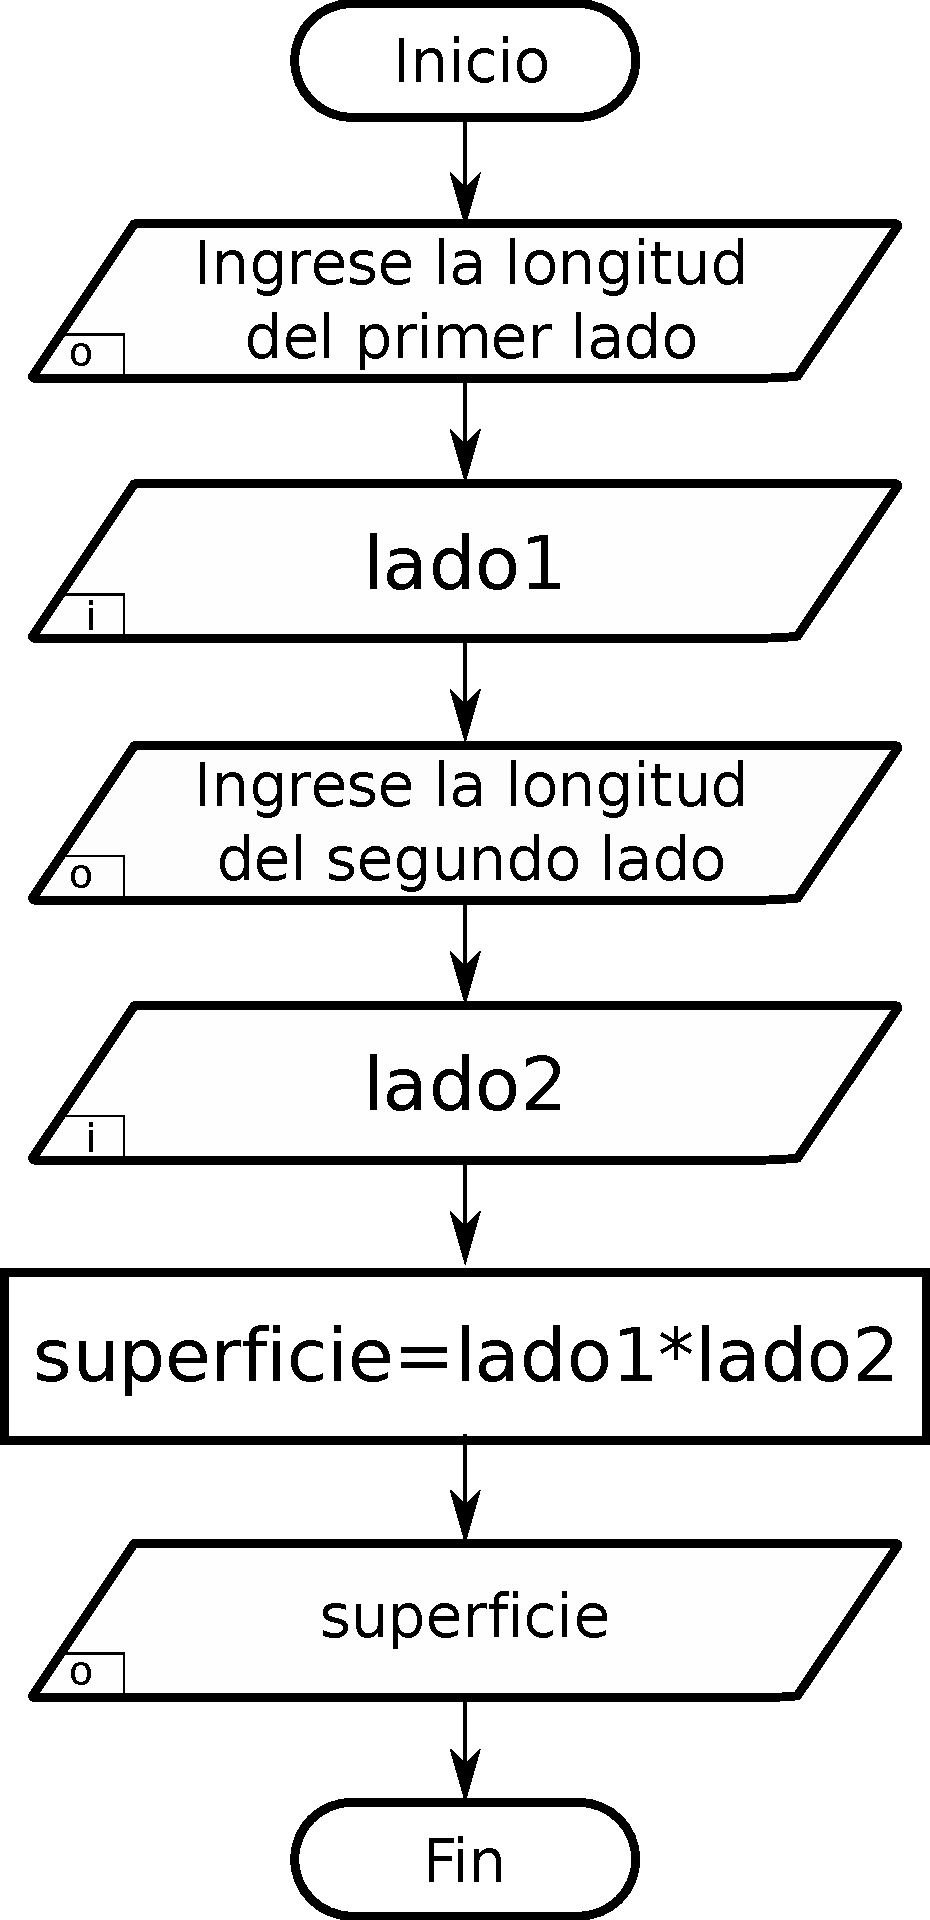
\includegraphics[height=80mm]{./img/ejercicio_1.pdf} 
\end{figure}

\pagebreak

\subsubsection{Ejercicio}
Escribir un algoritmo que solicite la edad de dos hermanos, muestre un mensaje indicando el mayor y su diferencia.

\subsubsection*{Solución}
\begin{lstlisting}[style=pseudocodigo]
imprimir: Ingrese la primera edad
leer:edad1
imprimir: Ingrese la segunda edad
leer: edad2
si edad1 > edad2 entonces
  imprimir: El primero es el mayor
si no
  imprimir: El segundo es el mayor
imprimir: diferencia
\end{lstlisting}

\begin{figure}[h!]
  \centering
  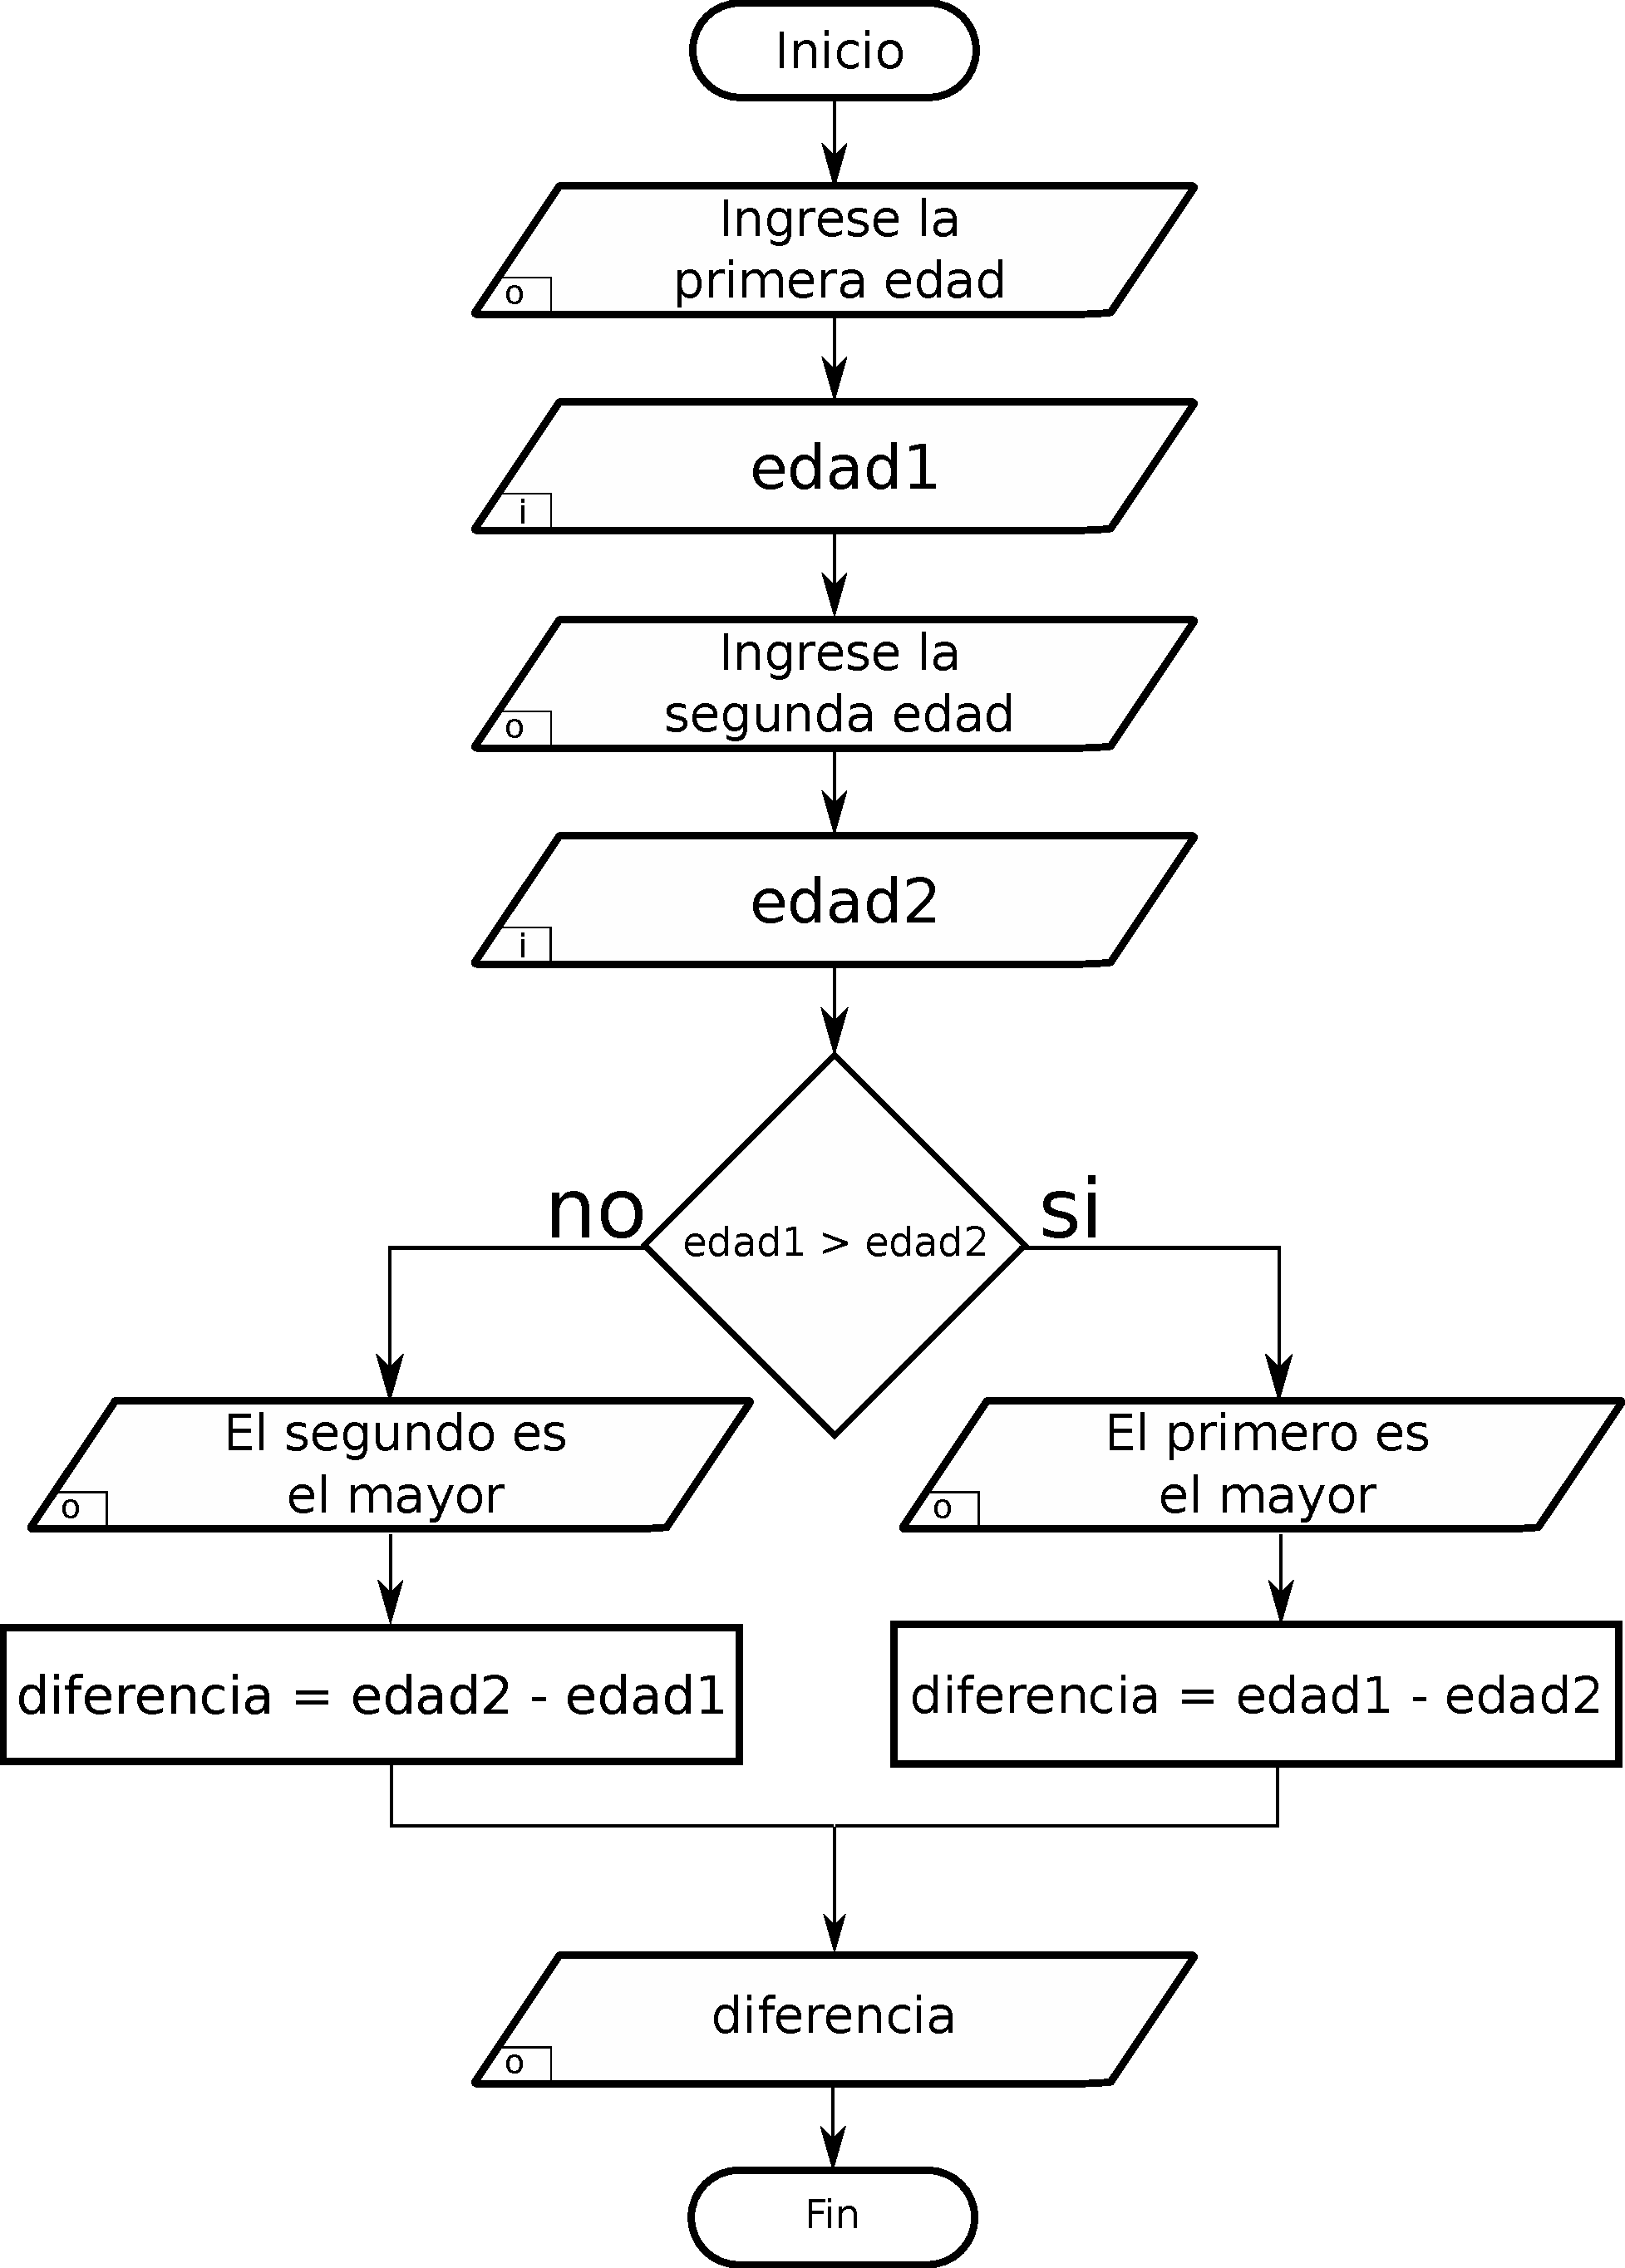
\includegraphics[height=150mm]{./img/ejercicio_2.pdf} 
\end{figure}

\pagebreak

\subsubsection{Ejercicio}
Escribir un algoritmo que imprima los números enteros desde el 0 hasta $N$. Donde el número $N$ es ingresado por el usuario.

\begin{lstlisting}[style=pseudocodigo]
imprimir: Ingrese N
leer: cantidad
para contador desde 0 hasta cantidad hacer
imprimir: contador
fin para
\end{lstlisting}

\begin{figure}[h!]
  \centering
  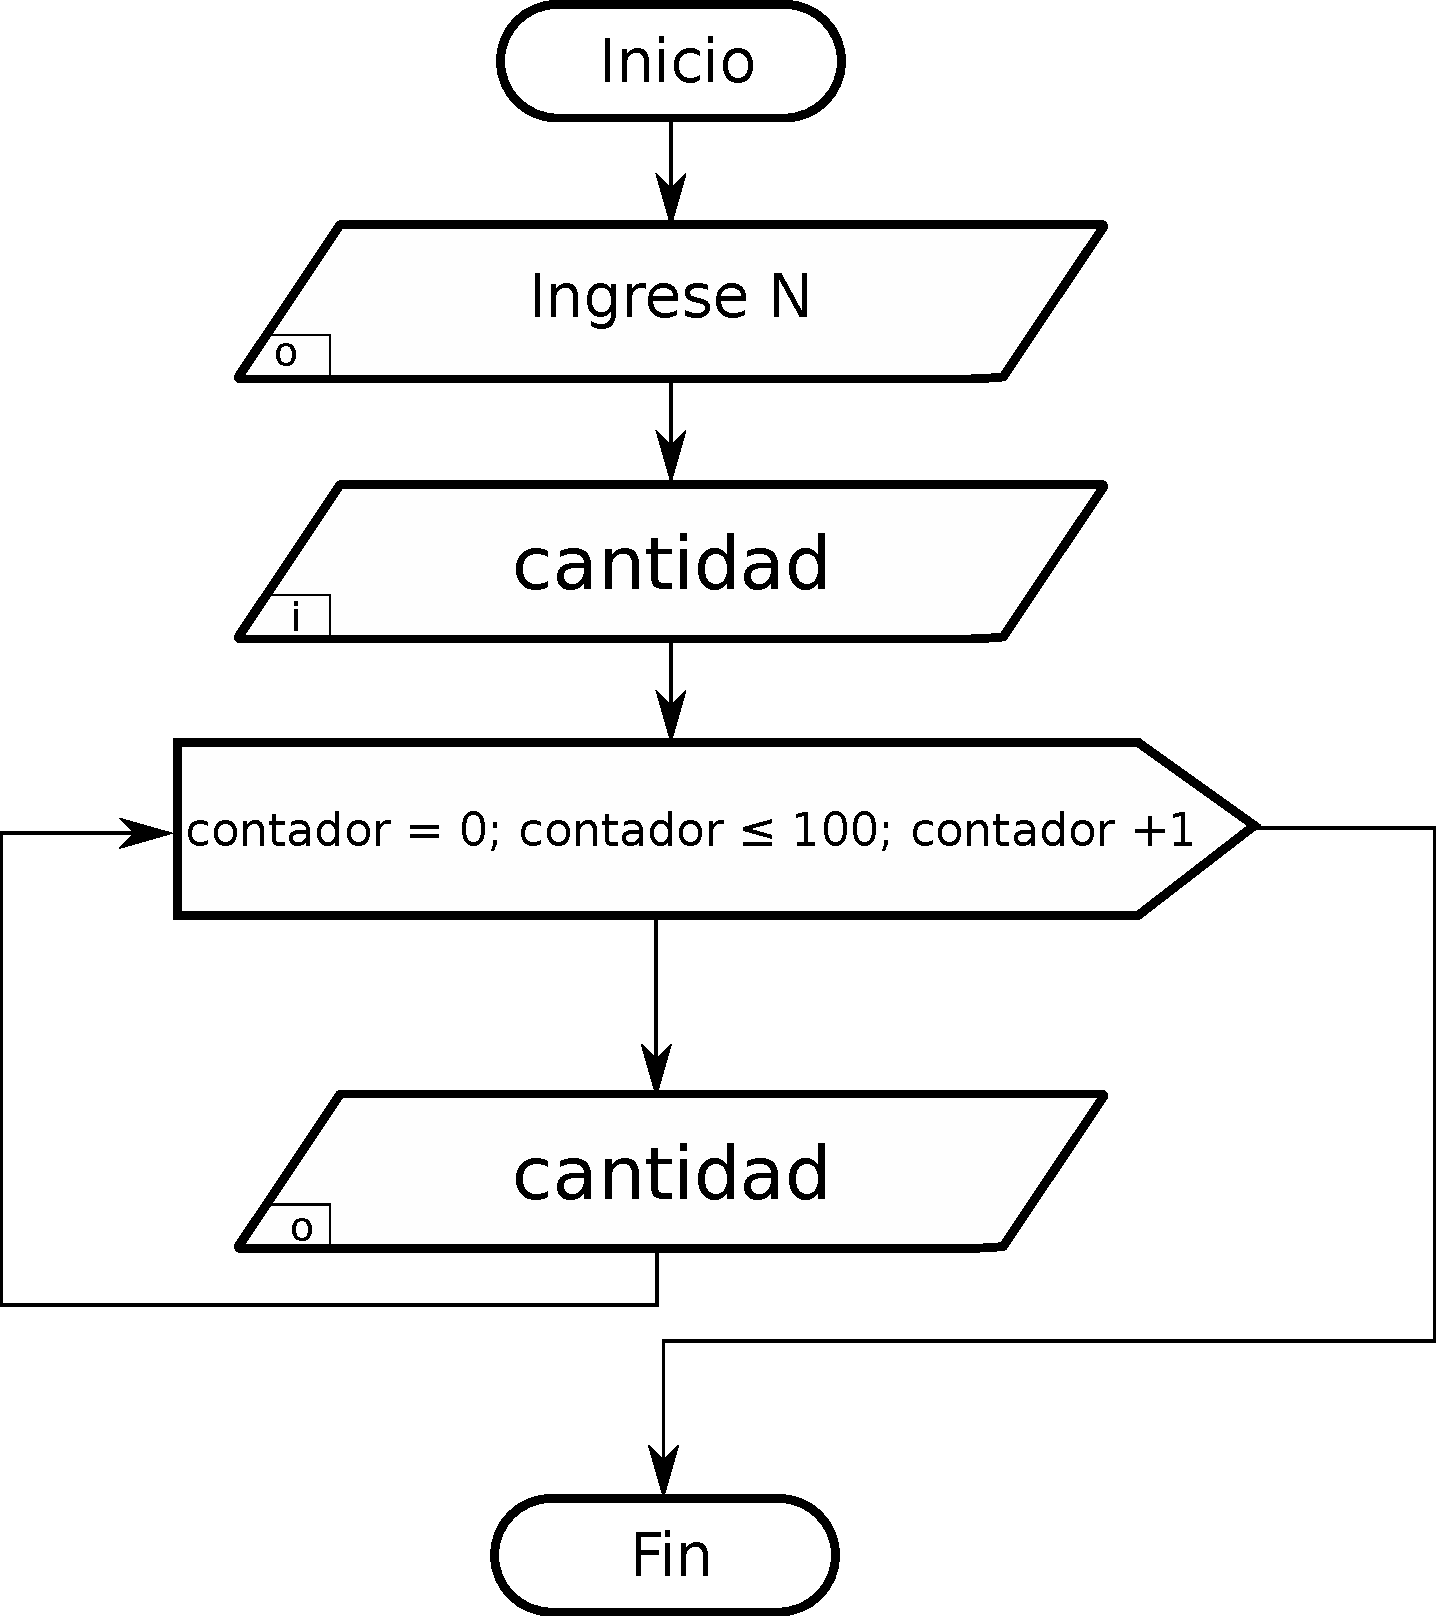
\includegraphics[height=110mm]{./img/ejercicio_3.pdf} 
  \caption{ejercicio 2 versión con bloque \textbf{para}}
\end{figure}

\pagebreak
\subsubsection{Preguntas:}
Completar los espacios en blanco:\\
\begin{enumerate}[a)]
  \item Todos los programas pueden ser escritos en términos de 3 secuencias de control:\underspace,\underspace,\underspace.
  \item La secuencia de control \underspace es utilizada para ejecutar una acción cuando es verdadera y otra acción cuando es falsa.
  \item La secuencia \underspace especifica que una o varias sentencias se ejecutarán repetidamente, mientras la condición sea verdadera.
\end{enumerate}


\pagebreak
% \subsubsection*{Selección}
\subsubsection{Ejercicio}
Escribir un algoritmo para calcular la distancia recorrida (m) por un móvil que se desplaza con velocidad constante (m/s) durante un tiempo (s). 
La velocidad y el tiempo serán ingresadas por el usuario.

\subsubsection{Ejercicio}
Escribir un algoritmo para obtener el promedio simple de un estudiante a partir de las tres notas parciales.
Las notas serán introducidas una a una por el usuario.

\subsubsection{Ejercicio}
En un local se hace un descuento del \%20 cuando la compra supera los \$ 1000. Escribir un algoritmo que calcule el precio a pagar por el cliente
teniendo como dato el valor de la compra.

\subsubsection{Ejercicio}
Escribir un algoritmo que determine si un número $n$ tiene tres cifras. El usuario debe ingresar el número $n$.

\subsubsection{Ejercicio}
Escribir un algoritmo que solicite ingresar dos números $n1$ y $n2$. Si el primero es mayor que el segundo mostrar la suma de ambos, por otro lado si el segundo es mayor al primero, mostrar el producto entre los números. En caso de que sean iguales imprimir ``Los números son iguales''.

% \subsubsection{Repetición}
\subsubsection{Ejercicio}
Escribir un programa que calcule la potencia $x={num1}^{num2}$, donde $num1$ y $num2$ son números enteros positivos ingresados por el usuario.

\subsubsection{Ejercicio}
Escribir un programa que calcule la suma de los primeros \textbf{n} números. El número \textbf{n} es un entero positivo, ingresado por el usuario.

\subsubsection{Ejercicio}
Escribir un algoritmo que imprima los número impares desde 0 hasta $N$. Donde $N$ es ingresado por el usuario.

\subsubsection{Ejercicio}
Escribir un algoritmo que determine la temperatura promedio de $N$ mediciones de temperatura. El usuario debe ingresar la cantidad $N$ y las $N$ mediciones. 

\subsubsection{Ejercicio}
Escribir un algoritmo que determine el mayor de 10 números ingresados. El usuario debe ingresar cada uno de los 10 números.

\subsubsection{Ejercicio}
Escribir un algoritmo que determine el mayor de $N$ números positivos ingresados. El usuario debe ingresar cada uno de los $N$ números. Para terminar se debe ingresar un -1.

\subsubsection{Ejercicio}
Escribir un algoritmo que solicite ingresar $N$ calificaciones de alumnos y determine la cantidad de aprobados, desaprobados y promocionados. 
El usuario debe ingresar el número $N$ y las $N$ calificaciones.

\underline{Según:}
\begin{itemize}
  \item Desaprobado: nota menor a 6
  \item Aprobado: nota mayor o igual a 6
  \item Promocionado: nota mayor o igual a 8
\end{itemize}

\subsubsection{Ejercicio}
Escribir de cuatro formas diferentes, sentencias en C que incrementen en 1 una variable \texttt{X}.

%--------------------------------------------------------------------------------
%--------------------------------------------------------------------------------
\subsection*{Control de flujo en lenguaje C}

\subsection*{if, if else}

\subsubsection{Solución}

\lstset{inputencoding=utf8/latin1}
\lstinputlisting[style=customc]{code/ejercicio0.c}
{\small
  \lstset{inputencoding=utf8/latin1}
  \lstinputlisting[backgroundcolor = \color{lightgray}]{code/ejercicio0_salida.mn}
}

\subsubsection{Ejercicio}
Realizar un programa que determine el mayor entre dos números ingresados por el usuario
{\small
  \lstset{inputencoding=utf8/latin1}
  \lstinputlisting[backgroundcolor = \color{lightgray}]{code/ejercicio1_salida.mn}
}

\subsubsection{Ejercicio}
Realizar un programa que determine el mayor entre tres números ingresados por el usuario. En caso de que trés o dos números sean iguales y los mayores, es indistinta la elección del mayor.
{\small
  \lstset{inputencoding=utf8/latin1}
  \lstinputlisting[backgroundcolor = \color{lightgray}]{code/ejercicio2_salida.mn}
}

\subsubsection{Ejercicio}
Realizar un programa que controle el encendido de un ventilador en base a la temperatura de encendido y la temperatura ambiente proporcionada por el usuario. Se debe imprimir en pantalla el estado del ventilador luego de ingresar los datos.
{\small
  \lstset{inputencoding=utf8/latin1}
  \lstinputlisting[backgroundcolor = \color{lightgray}]{code/ejercicio3_salida.mn}
}

\subsubsection{Ejercicio}
Realizar un programa que solicite ingresar las notas de dos parciales. Si desaprobó un parcial el programa debe solicitar ingresar la nota del recuperatorio. En base a las notas obtenidas calcular el promedio y determinar la condición académica (Promoción mayor 8, desaprobado menor a 6, lo demás aprobado). Solo se permite recuperar un solo parcial. La nota del recuperatorio se promedia con las notas del parcial y está permitido promocionar si recuperó.
{\small
  \lstset{inputencoding=utf8/latin1}
  \lstinputlisting[backgroundcolor = \color{lightgray}]{code/ejercicio4_salida.mn}
}

\subsubsection{Ejercicio}
Realizar un programa que dada la duracion en minutos de una llamada, permita calcular el costo,considerando:\\
-Hasta tres minutos el costo es 0.50 por minuto
-Por encima de tres minutos es 1.5 fijo más 0.2 por cada minuto adicional a los tres primeros
{\small
  \lstset{inputencoding=utf8/latin1}
  \lstinputlisting[backgroundcolor = \color{lightgray}]{code/ejercicio5_salida.mn}
}

%--------------------------------------------------------------------------------
%--------------------------------------------------------------------------------
\subsection*{Operadores \textbar\textbar, \&\&}
Realizar un programa que determine si 3 números ingresados son distintos entre ellos.
\subsubsection{Solución}

\lstset{inputencoding=utf8/latin1}
\lstinputlisting[style=customc]{code/ejercicio0.c}
{\small
  \lstset{inputencoding=utf8/latin1}
  % \lstinputlisting[backgroundcolor = \color{lightgray}]{code/ejercicio0_salida.mn}
}

\subsubsection{Ejercicio}
Realizar un programa que determine si un número ingresado por el usuario está en el rango 10-100. En caso de no estar en el rango, el programa de be informarlo y terminar. Si el número está dentro del rango, el programa debe determinar si el número es par.
{\small
  \lstset{inputencoding=utf8/latin1}
  \lstinputlisting[backgroundcolor = \color{lightgray}]{code/ejercicio1_operadores_salida.mn}
}

\subsubsection{Ejercicio}
Escribir un programa que determine el mayor de 3 números ingresados. Si los números son iguales, se debe imprimir un mensaje que lo indique.
{\small
  \lstset{inputencoding=utf8/latin1}
  \lstinputlisting[backgroundcolor = \color{lightgray}]{code/ejercicio2_operadores_salida.mn}
}

\subsubsection{Ejercicio}
Realizar un programa que solicite ingresar el valor nominal de resistencia (en ohms) y la tolerancia (valor entero en porcentaje). Una vez cargados estos valores, el programa debe solicitar al usuario que ingrese un valor de resistencia real y determine si la misma está dentro de los márgenes de tolerancia. 
{\small
  \lstset{inputencoding=utf8/latin1}
  \lstinputlisting[backgroundcolor = \color{lightgray}]{code/ejercicio3_operadores_salida.mn}
}

\subsubsection{Ejercicio}
Realizar un programa que determine si el caracter ingresado es un número o una letra. Ayuda: buscar ``tabla ASCII''.
{\small
  \lstset{inputencoding=utf8/latin1}
  \lstinputlisting[backgroundcolor = \color{lightgray}]{code/ejercicio4_operadores_salida.mn}
}

\subsubsection{Ejercicio}
Modificar el programa anterior para que ahora solicite ingresar el color de las bandas de colores y la medición real de la resisitencia. Con estos valores el programa debe determinar si se encuentra dentro de los valores de tolerancia o no. Considerar el caso de resistencias de 4 bandas de colores, donde las primeras tres indican el valor de resistencia y el cuarto la tolerancia (dorado $ \pm 5 $, plateado $\pm 10$, rojo $\pm 2$ y marrón $\pm 1$. Los colores de las bandas serán ingresados en forma de caracteres. Cada caracter representa un color.
\begin{itemize}
  \item \textbf{N}egro
  \item \textbf{M}arrón
  \item \textbf{R}ojo
  \item naran\textbf{J}a
  \item \textbf{A}marillo
  \item \textbf{V}erde
  \item a\textbf{Z}ul
  \item vio\textbf{L}eta
  \item \textbf{G}ris
  \item \textbf{B}lanco
  \item \textbf{D}orado
  \item \textbf{P}lateado
  \end{itemize}
{\small
  \lstset{inputencoding=utf8/latin1}
  \lstinputlisting[backgroundcolor = \color{lightgray}]{code/ejercicio5_operadores_salida.mn}
}

\subsection*{Estructura de selección múltiple switch-case}
\subsubsection{Ejercicio}
Realice un programa que determine el estado académico de un alumno en base a su promedio. El programa debe imprimir ``Promocionado'' si es mayor o igual a 8. ``Regular'' si es mayor o igual a 6 y menor que 8. Finalmente ``Desaprobado'' si es menor a 6.
Tener en cuenta que los valores posibles son únicamente entre 1 y 10.

\subsubsection{Ejercicio}
Realizar un programa en el cual se muestre al usuario un menú con cuatro operaciones matemáticas, a saber: suma, resta, división, multiplicación. El usuario debe ingresar el número de la operación y luego los dos operandos. Finalmente se debe mostrar en pantalla el resultado de la operación.

%--------------------------------------------------------------------------------
%--------------------------------------------------------------------------------
\subsection*{Estructuras repetitivas while}
Todos los ejercicios deben utilizar al menos una estructura \textbf{while}.
\subsubsection{Ejercicio}
Realizar un programa que solicite al usuario ingresar un número entre 0 y 100. Si el número está fuera del rango, el programa debe emitir una alerta y volver a pedir el número hasta que esté dentro del rango indicado.


\subsubsection{Ejercicio}
Realizar un programa que solicite al usuario ingresar un número par positivo. Si el número está fuera del rango, el programa debe emitir una alerta y volver a pedir el número hasta que esté dentro del rango indicado.


\subsubsection{Ejercicio}
Realizar un programa que solicite al usuario ingresar un número negativo. Si el número está fuera del rango, el programa debe emitir una alerta y volver a pedir el número hasta que esté dentro del rango indicado.

%--------------------------------------------------------------------------------
%--------------------------------------------------------------------------------
\subsection*{Estructuras repetitivas do..while}
Todos los ejercicios deben utilizar al menos una estructura \textbf{do..while}.
\subsubsection{Ejercicio}
Realizar un programa que solicite al usuario ingresar un número entre 0 y 100. Si el número está fuera del rango, el programa debe emitir una alerta y volver a pedir el número hasta que esté dentro del rango indicado.

\subsubsection{Ejercicio}
Realizar un programa que solicite al usuario ingresar un número par positivo. Si el número está fuera del rango, el programa debe emitir una alerta y volver a pedir el número hasta que esté dentro del rango indicado.

\subsubsection{Ejercicio}
Realizar un programa que solicite al usuario ingresar un impar. Si el número está fuera del rango, el programa debe emitir una alerta y volver a pedir el número hasta que esté dentro del rango indicado.

%--------------------------------------------------------------------------------
%--------------------------------------------------------------------------------
\subsection*{Estructura repetitiva for}
Todos los ejercicios deben utilizar al menos una estructura \textbf{for}.
Algunos ejercicios pueden requerir utilizar estructuras de condición.

\subsubsection{Ejercicio}
Realizar un programa que imprima los números desde el 5 hasta el 0 y luego vuelva hasta el 5 como en el siguiente ejemplo (se debe utilizar al menos una estructura for)

\subsubsection{Solución}

\lstset{inputencoding=utf8/latin1}
\lstinputlisting[style=customc]{code/ejercicio0.c}
{\small
  \lstset{inputencoding=utf8/latin1}
  \lstinputlisting[backgroundcolor = \color{lightgray}]{code/ejercicio0_salida.mn}
}
\subsubsection{Solución (con un solo for)}
\lstinputlisting[style=customc]{code/ejercicio0_un.c}
{\small
  \lstset{inputencoding=utf8/latin1}
  \lstinputlisting[backgroundcolor = \color{lightgray}]{code/ejercicio0_salida.mn}
}

\subsubsection{Preguntas}
\begin{itemize}
  \item La iteración controlada por contador también se conoce como iteración \underspace porque se sabe de antemano cuántas veces se ejecutará el bucle.
  \item La iteración controlada por centinela también se conoce como iteración \underspace porque no se sabe de antemano cuántas veces se ejecutará el bucle.
  \item En la iteración controlada por contador, se usa un(una)\underspace  para contar el número de veces que se debe repetir un grupo de instrucciones.
\end{itemize}

\subsubsection{Analizar código}
Encontrar el error en las siguientes códigos:
\begin{enumerate}
  \item .
  \lstinputlisting[style=customc]{code/ejercicio_rep_a.c}
  \item .
  \lstinputlisting[style=customc]{code/ejercicio_rep_b.c}
\end{enumerate}

\subsubsection{Ejercicio}
Modificar el programa anterior para que imprima la progresión de números partiendo de un número $n$ positivo ingresado por el usuario. 
{\small
  \lstset{inputencoding=utf8/latin1}
  \lstinputlisting[backgroundcolor = \color{lightgray}]{code/ejercicio1_rep_salida.mn}
}

\subsubsection{Ejercicio}
Realizar un programa que utilice una estructura \textbf{for} e imprima la siguiente salida:
{\small
  \lstset{inputencoding=utf8/latin1}
  \lstinputlisting[backgroundcolor = \color{lightgray}]{code/ejercicio2_rep_salida.mn}
}

\subsubsection{Ejercicio}
Realizar un programa que utilice una entructura \textbf{for} e imprima la siguiente tabla:
{\small
  \lstset{inputencoding=utf8/latin1}
  \lstinputlisting[backgroundcolor = \color{lightgray}]{code/ejercicio3_rep_salida.mn}
}

\subsubsection{Ejercicio}
Realizar un programa que utilice dos entructuras \textbf{for} para imprimir una matriz, donde la cantidad de filas y columnas son ingresados por el usuario como la siguiente:
{\small
  \lstset{inputencoding=utf8/latin1}
  \lstinputlisting[backgroundcolor = \color{lightgray}]{code/ejercicio4_rep_salida.mn}
}

\subsubsection{Ejercicio}
Escribir un programa que imprima todos los números enteros pares entre el 0 y $n$, donde $n$ es un número entero ingresado por el usuario.
{\small
  \lstset{inputencoding=utf8/latin1}
  \lstinputlisting[backgroundcolor = \color{lightgray}]{code/ejercicio5_rep_salida.mn}
}

\subsubsection{Ejercicio}
Escribir un programa que determine el mayor de 10 números enteros ingresados por el usuario.
{\small
  \lstset{inputencoding=utf8/latin1}
  \lstinputlisting[backgroundcolor = \color{lightgray}]{code/ejercicio6_rep_salida.mn}
}

\subsubsection{Ejercicio}
Modificar el programa del ejercicio anterior para que determine también el mínimo número ingresado.
{\small
  \lstset{inputencoding=utf8/latin1}
  \lstinputlisting[backgroundcolor = \color{lightgray}]{code/ejercicio7_rep_salida.mn}
}

\subsubsection{Ejercicio}
Realizar un programa que calcule la tabla de multiplicar de un número $n$ ingresado por el usuario.
{\small
  \lstset{inputencoding=utf8/latin1}
  \lstinputlisting[backgroundcolor = \color{lightgray}]{code/ejercicio8_rep_salida.mn}
}

\subsubsection{Ejercicio}
Realizar un programa que calcule el factorial de un número $n$ ingresado por el usuario. Donde $0<n<10$.
{\small
  \lstset{inputencoding=utf8/latin1}
  \lstinputlisting[backgroundcolor = \color{lightgray}]{code/ejercicio9_rep_salida.mn}
}

\subsubsection{Ejercicio }
Realizar un programa que calcule la potencia $m$ de número $n$, donde $m$ y $n$ son ingresado por el usuario. Operación: $n^m$.
{\small
  \lstset{inputencoding=utf8/latin1}
  \lstinputlisting[backgroundcolor = \color{lightgray}]{code/ejercicio10_rep_salida.mn}
}


\subsection*{\underline{Ejercicios de cierre}}
\subsubsection{Cálculo límites de frecuencia cardíaca}

Según la American Heart Association (AHA), la fórmula para calcular su frecuencia cardíaca máxima en ritmos por minuto es 220 menos su edad en años.
Su frecuencia cardíaca objetivo es un rango del 50-85\% de su frecuencia cardíaca máxima.
Nota: Estas fórmulas son estimadas por la AHA.
Las velocidades cardíacas máximas y objetivo pueden variar según la salud, el estado físico y el género del individuo.
Siempre consulte a un médico o un profesional de salud calificado antes de comenzar o modificar un programa de ejercicios.
Cree un programa que lea el cumpleaños del usuario y el día actual (cada uno que consiste en el mes, el día y el año).
Su programa debe calcular y mostrar la edad de la persona (en años), la frecuencia cardíaca máxima de la persona y el rango de tasa de corazón objetivo de la persona.

Mientras hace ejercicio, puede usar un monitor de frecuencia cardíaca para ver que su frecuencia cardíaca permanece dentro de un rango seguro sugerido por sus entrenadores y médicos

\subsubsection{Cálculo creciemiento de población mundial}
La población mundial ha crecido considerablemente a lo largo de los siglos.
El crecimiento continuo eventualmente podría desafiar los límites del aire transpirable, el agua potable, las tierras de cultivo cultivables y otros recursos limitados.
Existe evidencia de que el crecimiento se ha desacelerado en los últimos años y que la población mundial podría alcanzar algún tiempo en este siglo, luego comenzar a disminuir.
Para este ejercicio, investigue en internet sobre la población mundial y su crecimiento.
Asegúrese de buscar varios puntos de vista.
Obtenga estimaciones para la población mundial actual y su tasa de crecimiento (el porcentaje por el cual es probable que aumente este año).
Escriba un programa que calcule el crecimiento de la población mundial cada año durante los próximos 75 años, utilizando la suposición simplificadora de que la tasa de crecimiento actual se mantendrá constante.
Imprima los resultados en una tabla.
La primera columna debe mostrar el año del año 1 al año 75.
La segunda columna debe mostrar la población mundial anticipada a finales de ese año.
La tercera columna debe mostrar el aumento numérico en la población mundial que ocurriría ese año.
Usando sus resultados, determine el año en que la población sería el doble de lo que es hoy, si la tasa de crecimiento de este año persistiera.

